\chapter{Experimental Design}

\section{Dataset Preprocessing}

This section describes the preprocessing steps applied to the time series datasets used in this study. Initially, we had access to four different datasets: two containing measurements taken on sand and two on clay. Each dataset included various variables representing different environmental conditions and characteristics. However, during the data exploration phase, significant inconsistencies were identified in three of the datasets.

The errors detected included abrupt increases in the values of certain variables from one day to the next. In the sand datasets, it was observed that for diameter measurements, the values unexpectedly doubled or tripled overnight. This phenomenon could be explained by a possible change of sensors, which might have altered the measurements without prior notice.

\begin{figure}[htbp]
    \centering
    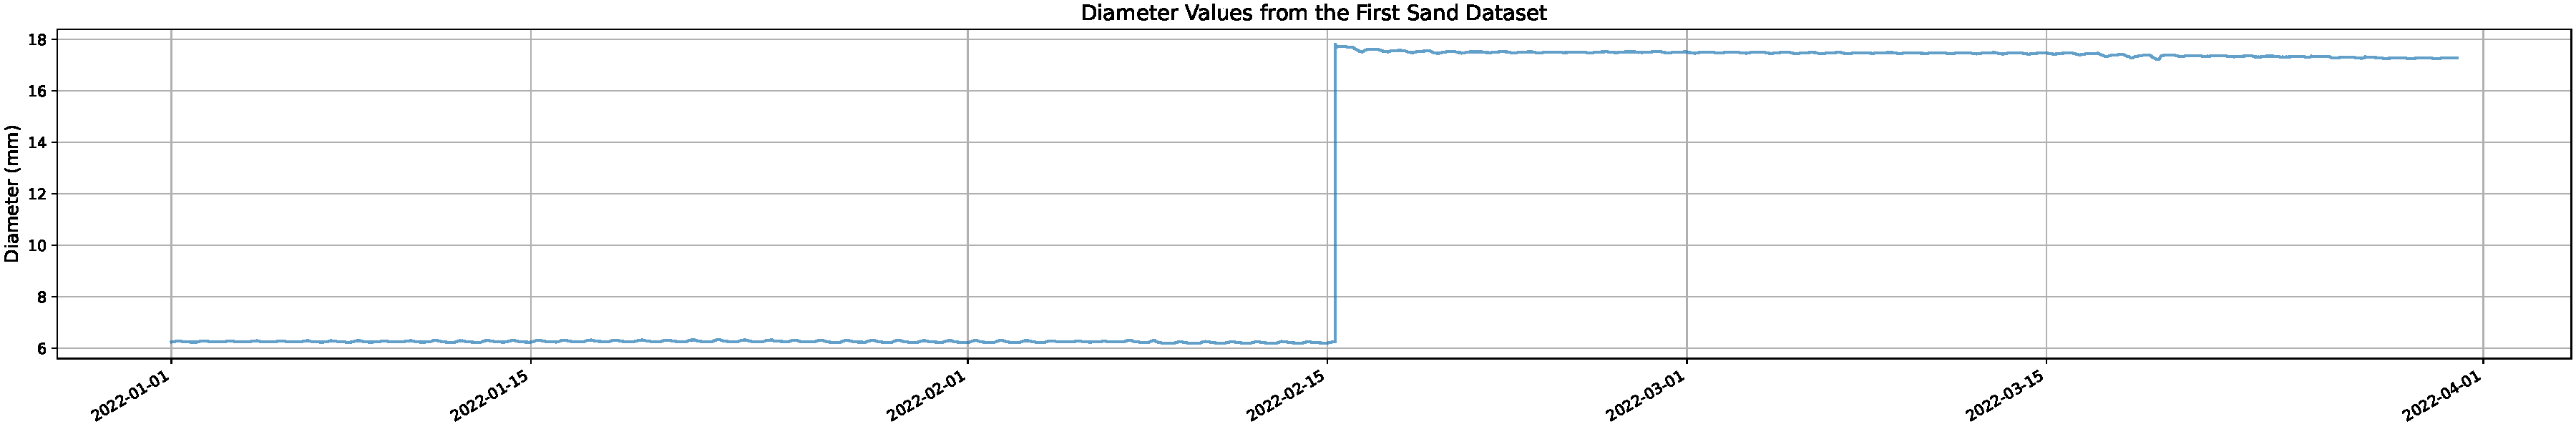
\includegraphics[width=15 cm]{5_ChapterDesign/figuras/1_DatasetIssues/Diameter_Sand_1}
    \caption{Example of Diameter Measurement Error in the First Sand Dataset}
    \LABFIG{FIG}
    \end{figure}

Similarly, the data related to light intensity showed sudden variations in lumens. In this case, it is likely that the sensor was either cleaned or repositioned, which could have caused a significant change in light measurements from one day to the next. The following image illustrates an example of these abrupt changes:

\begin{figure}[htbp]
    \centering
    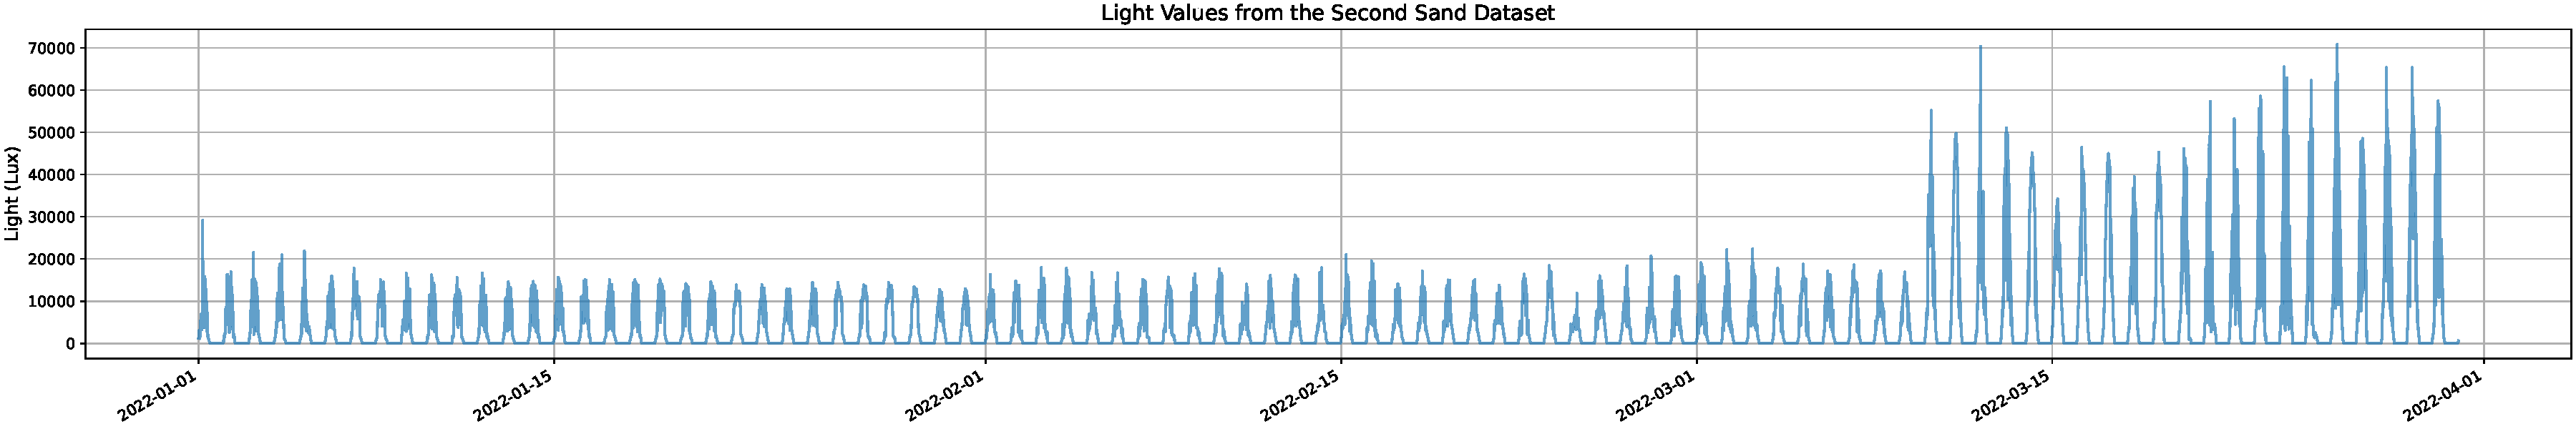
\includegraphics[width=15 cm]{5_ChapterDesign/figuras/1_DatasetIssues/Light_Sand_2}
    \caption{Example of Light Measurement Error in the Second Sand Dataset}
    \LABFIG{FIG}
    \end{figure}

Due to these inconsistencies and after a thorough evaluation of the data, we decided to use one of the clay datasets, which presented more reasonable and consistent measurements over time. This dataset was selected for further analysis as it offered a more stable and reliable framework for studying time series data.

However, even the selected dataset required significant preprocessing to transform its structure and ensure data quality. This preprocessing process included steps such as normalizing values, handling missing data, and removing potential outliers. The detailed steps carried out in this phase are presented below.

\subsection{Structure}

The initial dataset provided by Ornavera was in the \texttt{.mat} format, which is commonly used for MATLAB. To facilitate data analysis and manipulation in Python, it was necessary to convert this data into a \texttt{.csv} file format. This conversion was advantageous because \texttt{.csv} files are universally supported and can be easily imported into Python libraries such as Pandas, making data manipulation and analysis straightforward. Additionally, CSV files are text-based, making them easy to inspect and modify with a simple text editor, and they offer efficiency benefits for large datasets due to their simple structure, which can be quickly parsed by Python libraries.

To perform the conversion, we wrote a MATLAB function named \texttt{mat\_to\_csv}, which loads the data from the \texttt{.mat} file, eliminates unnecessary fields, and writes the cleaned data to a \texttt{.csv} file. The function specifically targeted fields that were not relevant to our analysis, such as various identifiers and redundant measurements. Removing these fields helped streamline the dataset, ensuring that it was focused on the variables that were of interest for our study.

\begin{lstlisting}[language=Matlab,caption={MATLAB function to convert .mat file to .csv}, label=lst:mat_to_csv]
function mat_to_csv(mat_file, csv_file)
    % Load the data from the .mat file
    load(mat_file, 'val');
    
    % Eliminate the fields we are not interested in
    fields_to_eliminate = {'rid', 'cid','lid','vpd1','dd1','wtlux','alux','ecb1','ecp1','st2', 'p2', 'ec2', 'vwc2', 'ecb2', 'ecp2', 'st3', 'p3', 'ec3', 'vwc3', 'ecb3', 'ecp3','par','dli'};
    val_cleaned = val; % Create a copy of the original structure
    for i = 1:numel(fields_to_eliminate)
        val_cleaned = rmfield(val_cleaned, fields_to_eliminate{i});
    end
    
    % Convert the data from a structure to a table
    val_table = struct2table(val_cleaned);
    
    % Change the field names of the table
    new_names = {'Identificator', 'Date', 'Month','Day','Year','Hour','Minute','Second','Temperature','Relative_humidity', 'Light', 'Soil_temperature', 'Permittivity', 'Electroconductivity', 'Volumetric_water_content', 'Diameter', 'Battery_voltage'};
    val_table.Properties.VariableNames = new_names;
    
    % Write the data to a .csv file
    writetable(val_table, csv_file, 'Delimiter', ';');
end
\end{lstlisting}

The code effectively transformed the data from a complex structure into a more usable format by converting it into a table and renaming the fields to be more descriptive. The \texttt{.csv} file was then generated with a delimiter suitable for easy parsing in Python. This preparation step was crucial in setting the stage for efficient data handling and analysis in the subsequent phases of the project.

\subsection{Signal smoothing}

To achieve the signal smoothing, we use a Savitzky-Golay filter with a window size of 11 and a polynomial order of 2. In this case, we start with the data signal after removing the initial slope. The window size is set to 11, meaning that 11 adjacent data points are used to calculate each smoothed value. This implies that the filter takes these 11 points and fits a second-degree polynomial, also known as a parabola, to the data within each window, allowing the signal to be smoothed without losing its essential characteristics.

The \texttt{savgol\_filter} function generates a smoothed version of the input signal. By applying this filter, the smoothed signal exhibits a significant reduction in noise, making it more continuous and less fluctuating than the original signal. The smoothing process enhances the visualization and analysis of the underlying trends in the data, allowing important features to stand out more clearly. This can be clearly observed in the graphs presented below.


\begin{figure}[htbp]
    \centering
    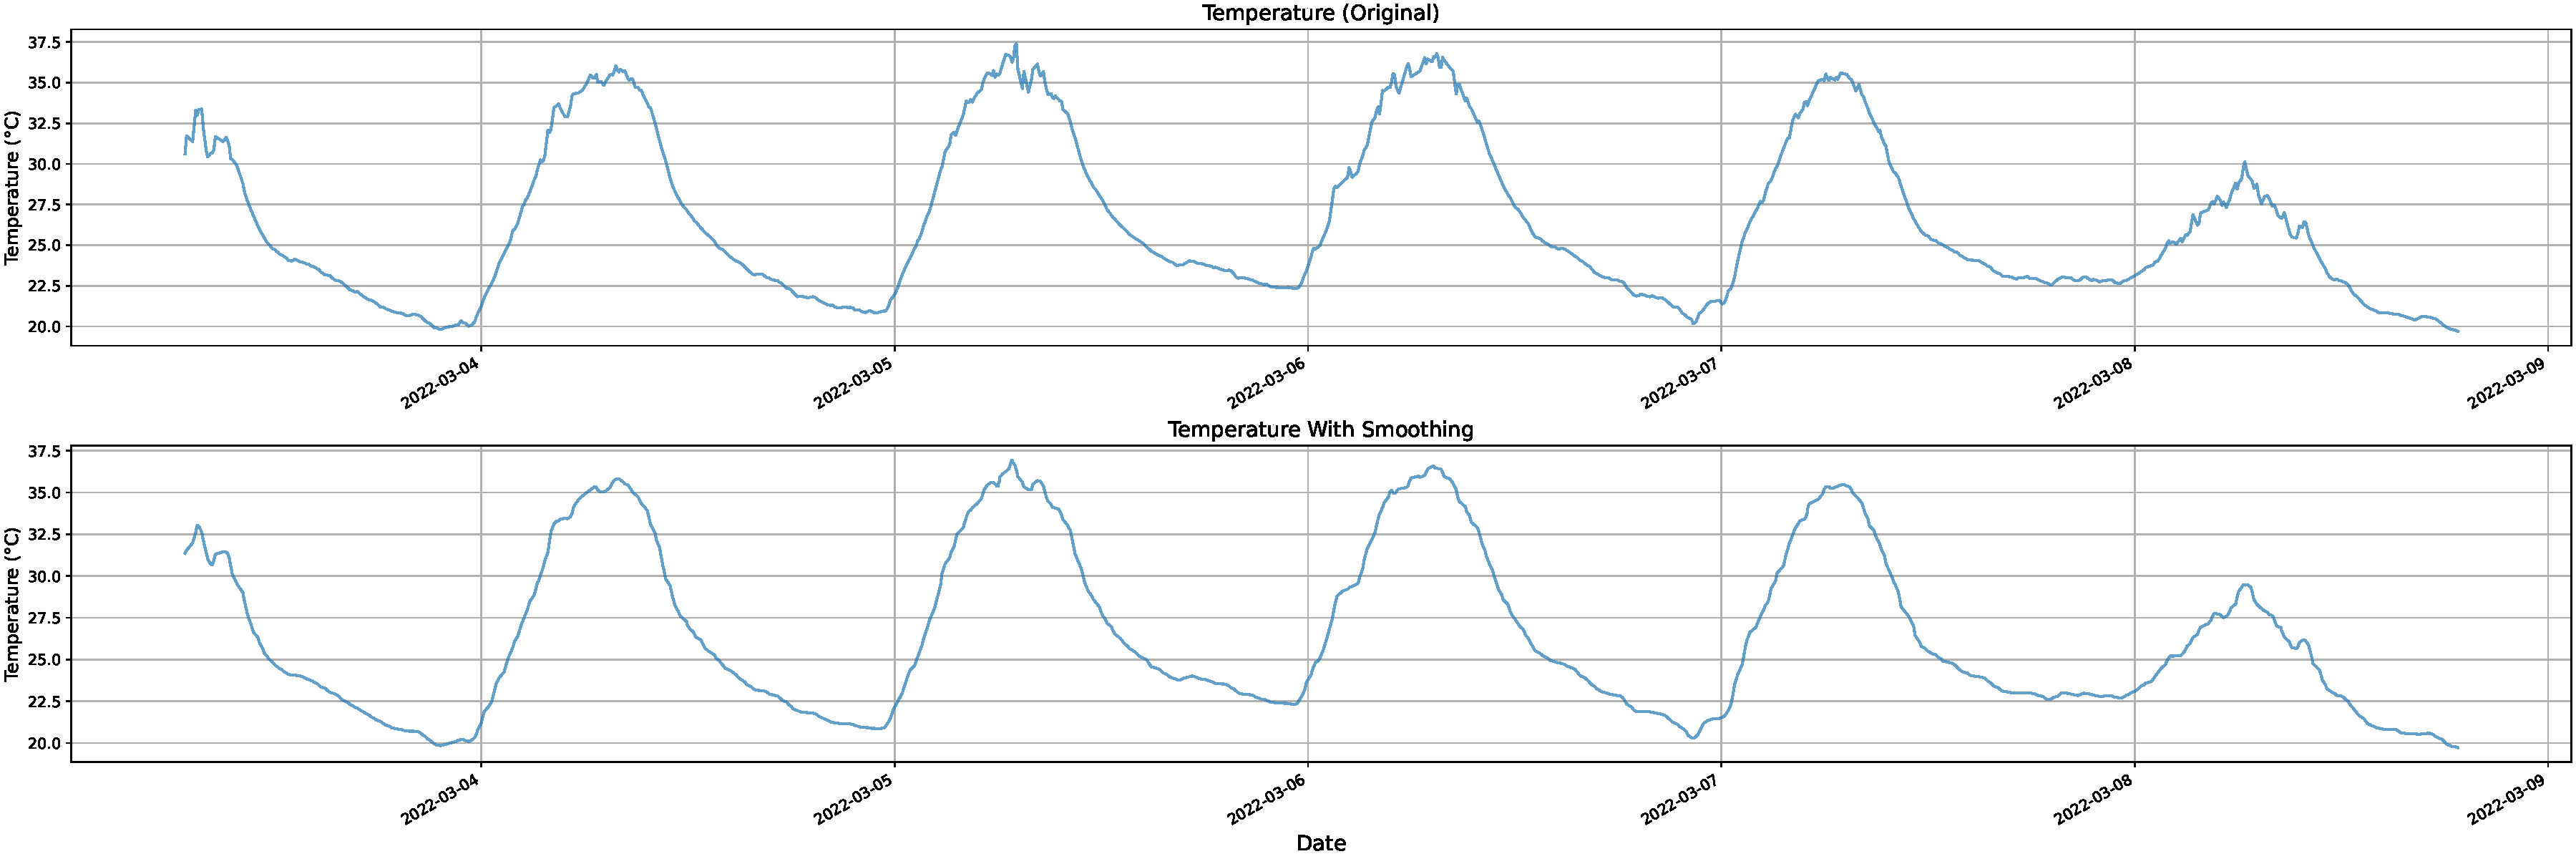
\includegraphics[width=15 cm]{5_ChapterDesign/figuras/2_Smoothing/Smoothing_Temperature}
    \caption{Original Temperature data (top) versus the Temperature smoothed data (bottom) after applying a Savitzky-Golay filter}
    \LABFIG{FIG}
\end{figure}

\begin{figure}[htbp]
    \centering
    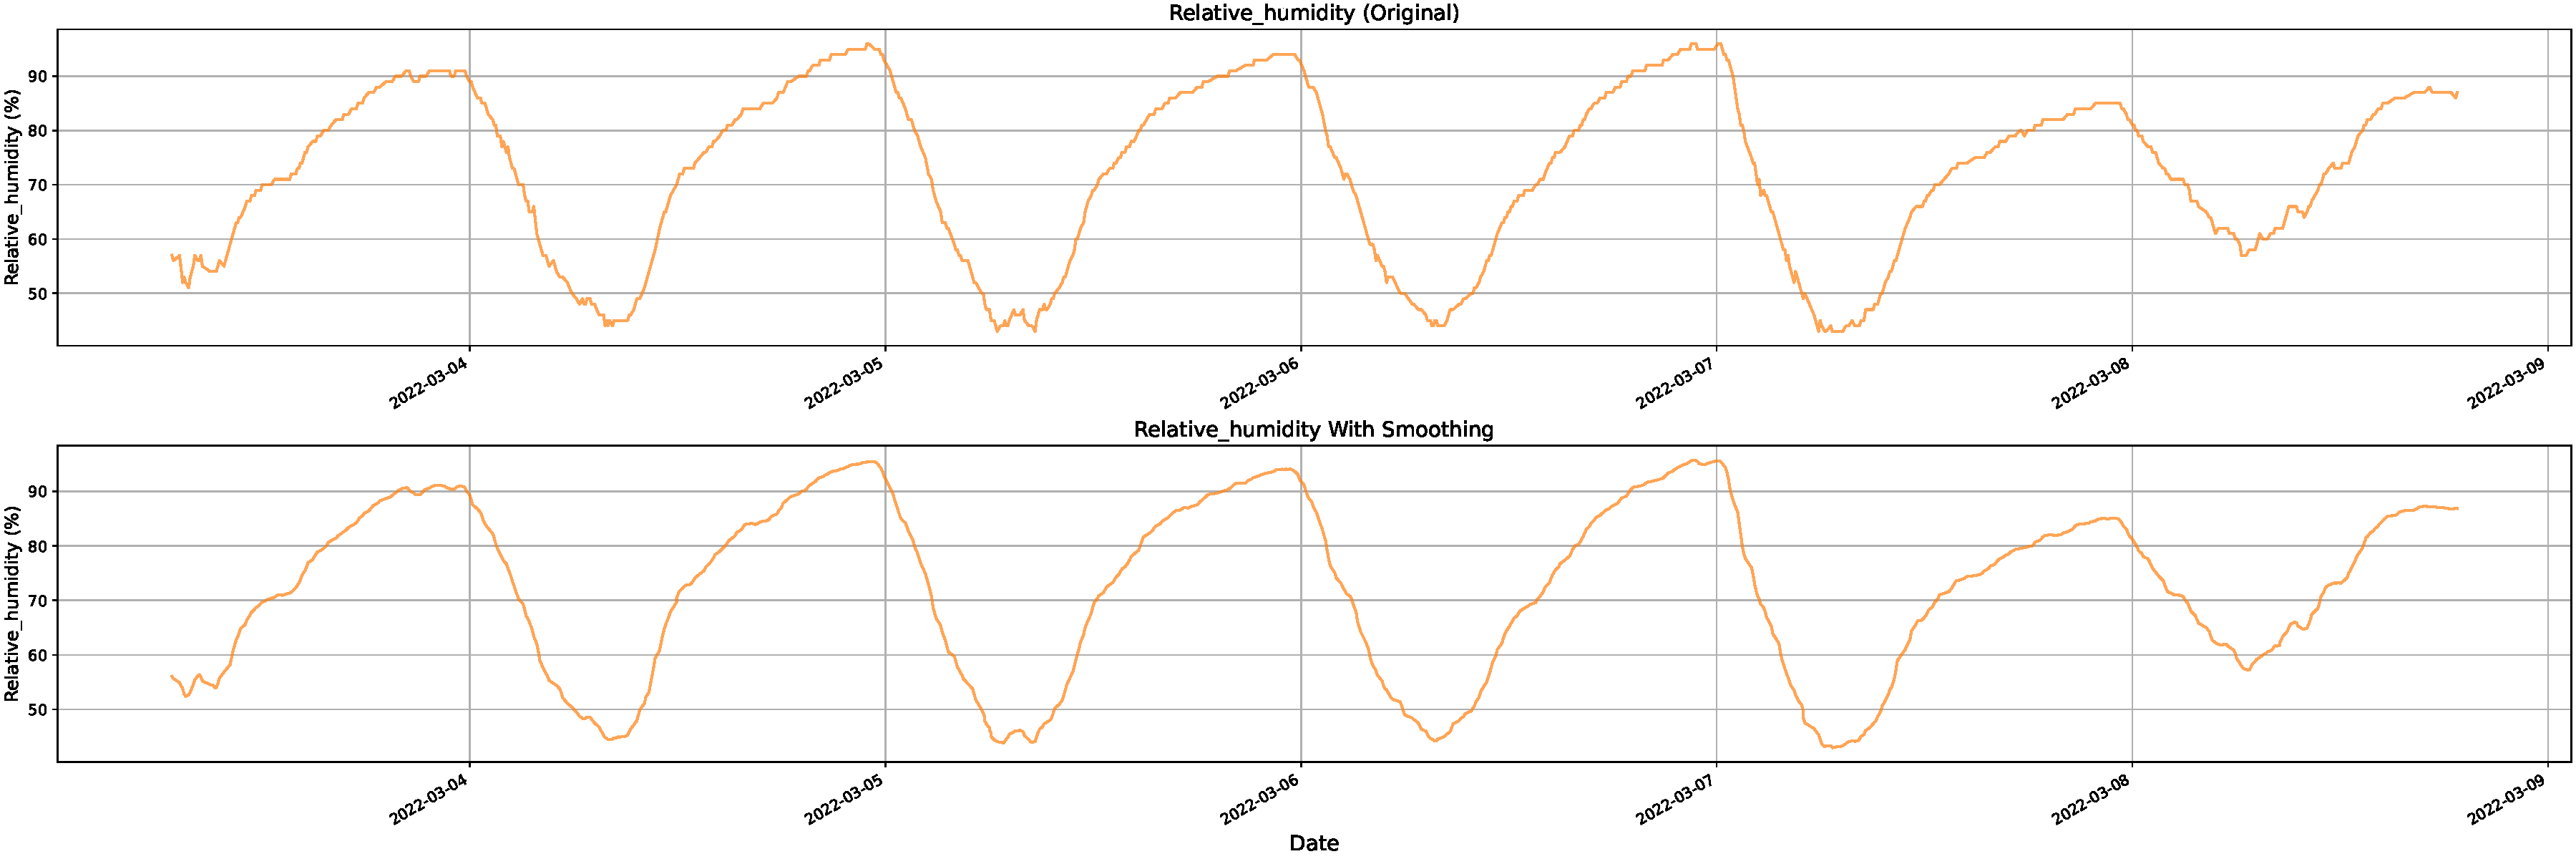
\includegraphics[width=15 cm]{5_ChapterDesign/figuras/2_Smoothing/Smoothing_Relative_humidity}
    \caption{Original Relative humidity data (top) versus the Relative humidity smoothed data (bottom) after applying a Savitzky-Golay filter}
    \LABFIG{FIG}
\end{figure}

\begin{figure}[htbp]
    \centering
    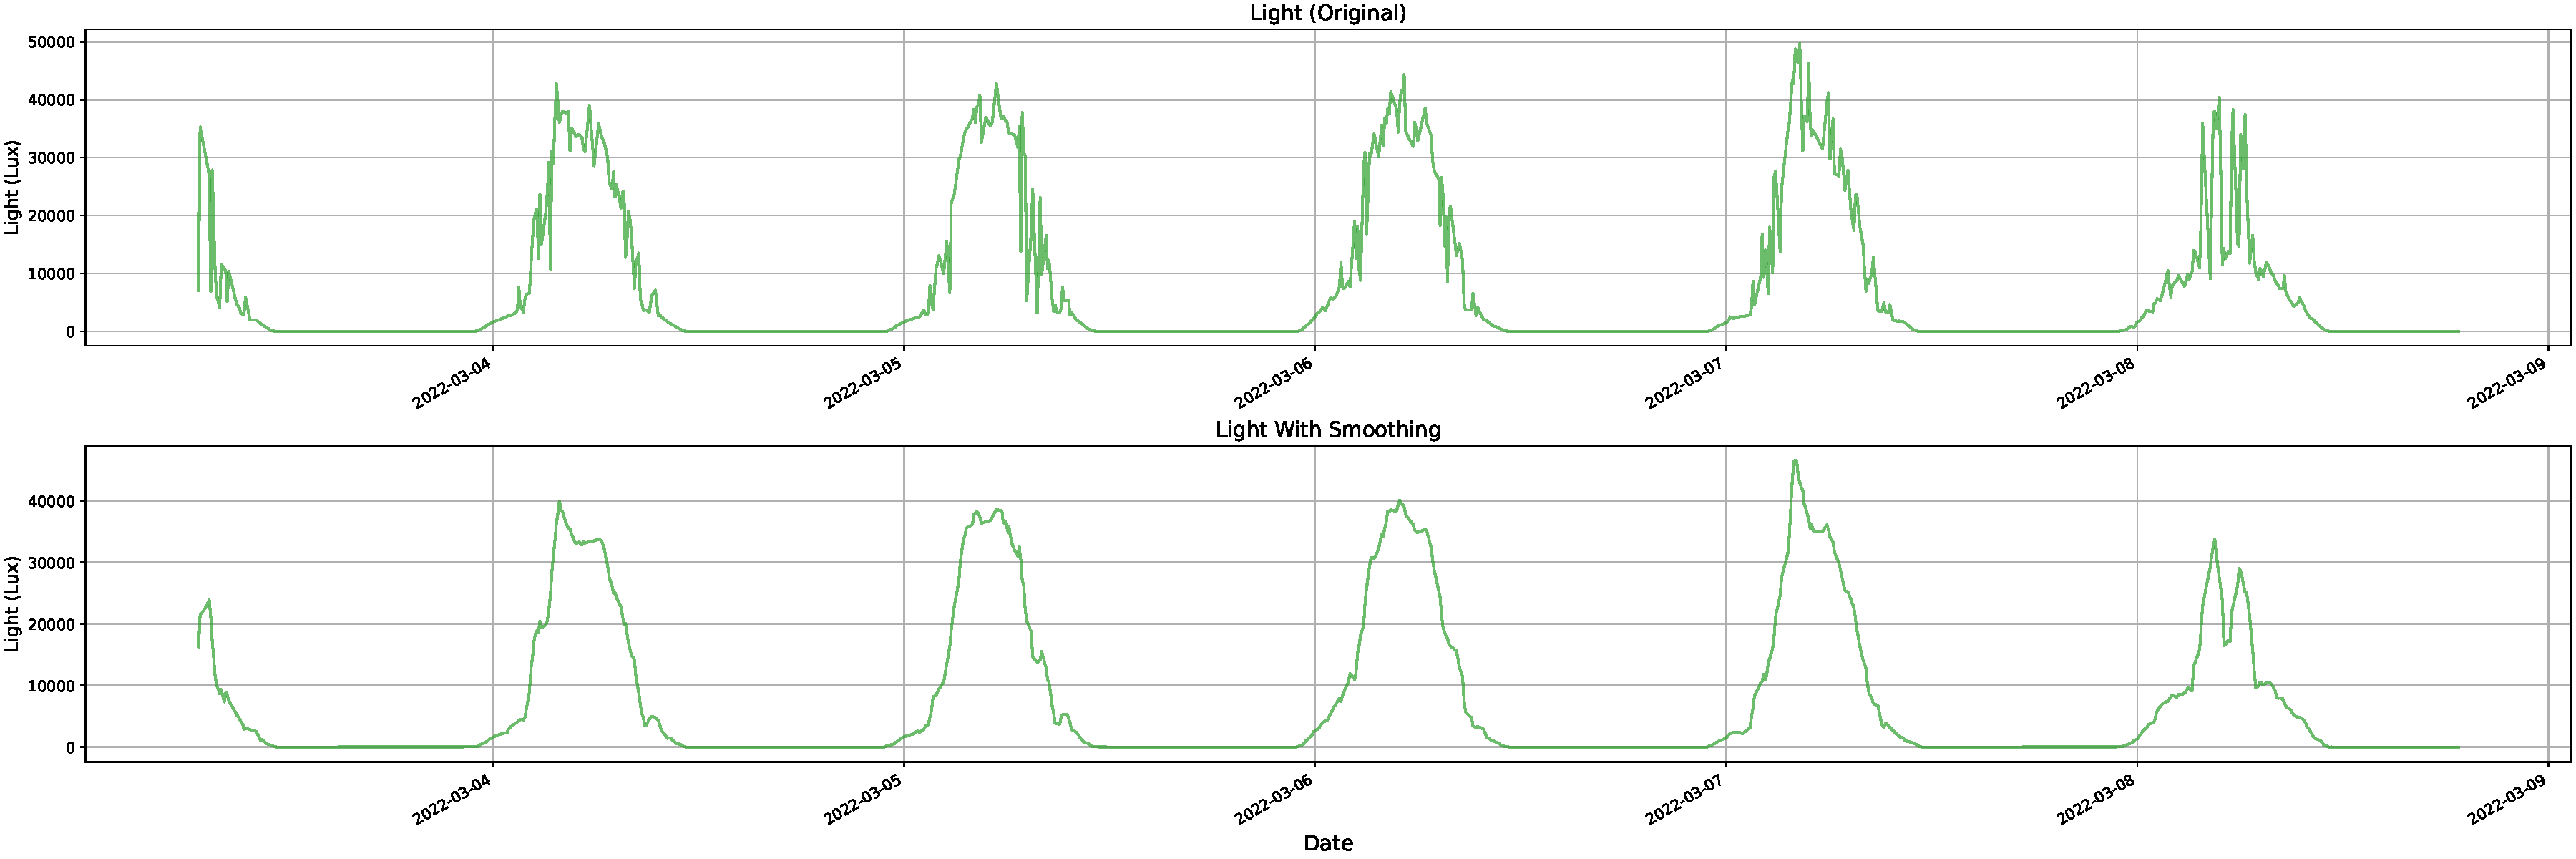
\includegraphics[width=15 cm]{5_ChapterDesign/figuras/2_Smoothing/Smoothing_Light}
    \caption{Original Light data (top) versus the Light smoothed data (bottom) after applying a Savitzky-Golay filter}
    \LABFIG{FIG}
\end{figure}

\begin{figure}[htbp]
    \centering
    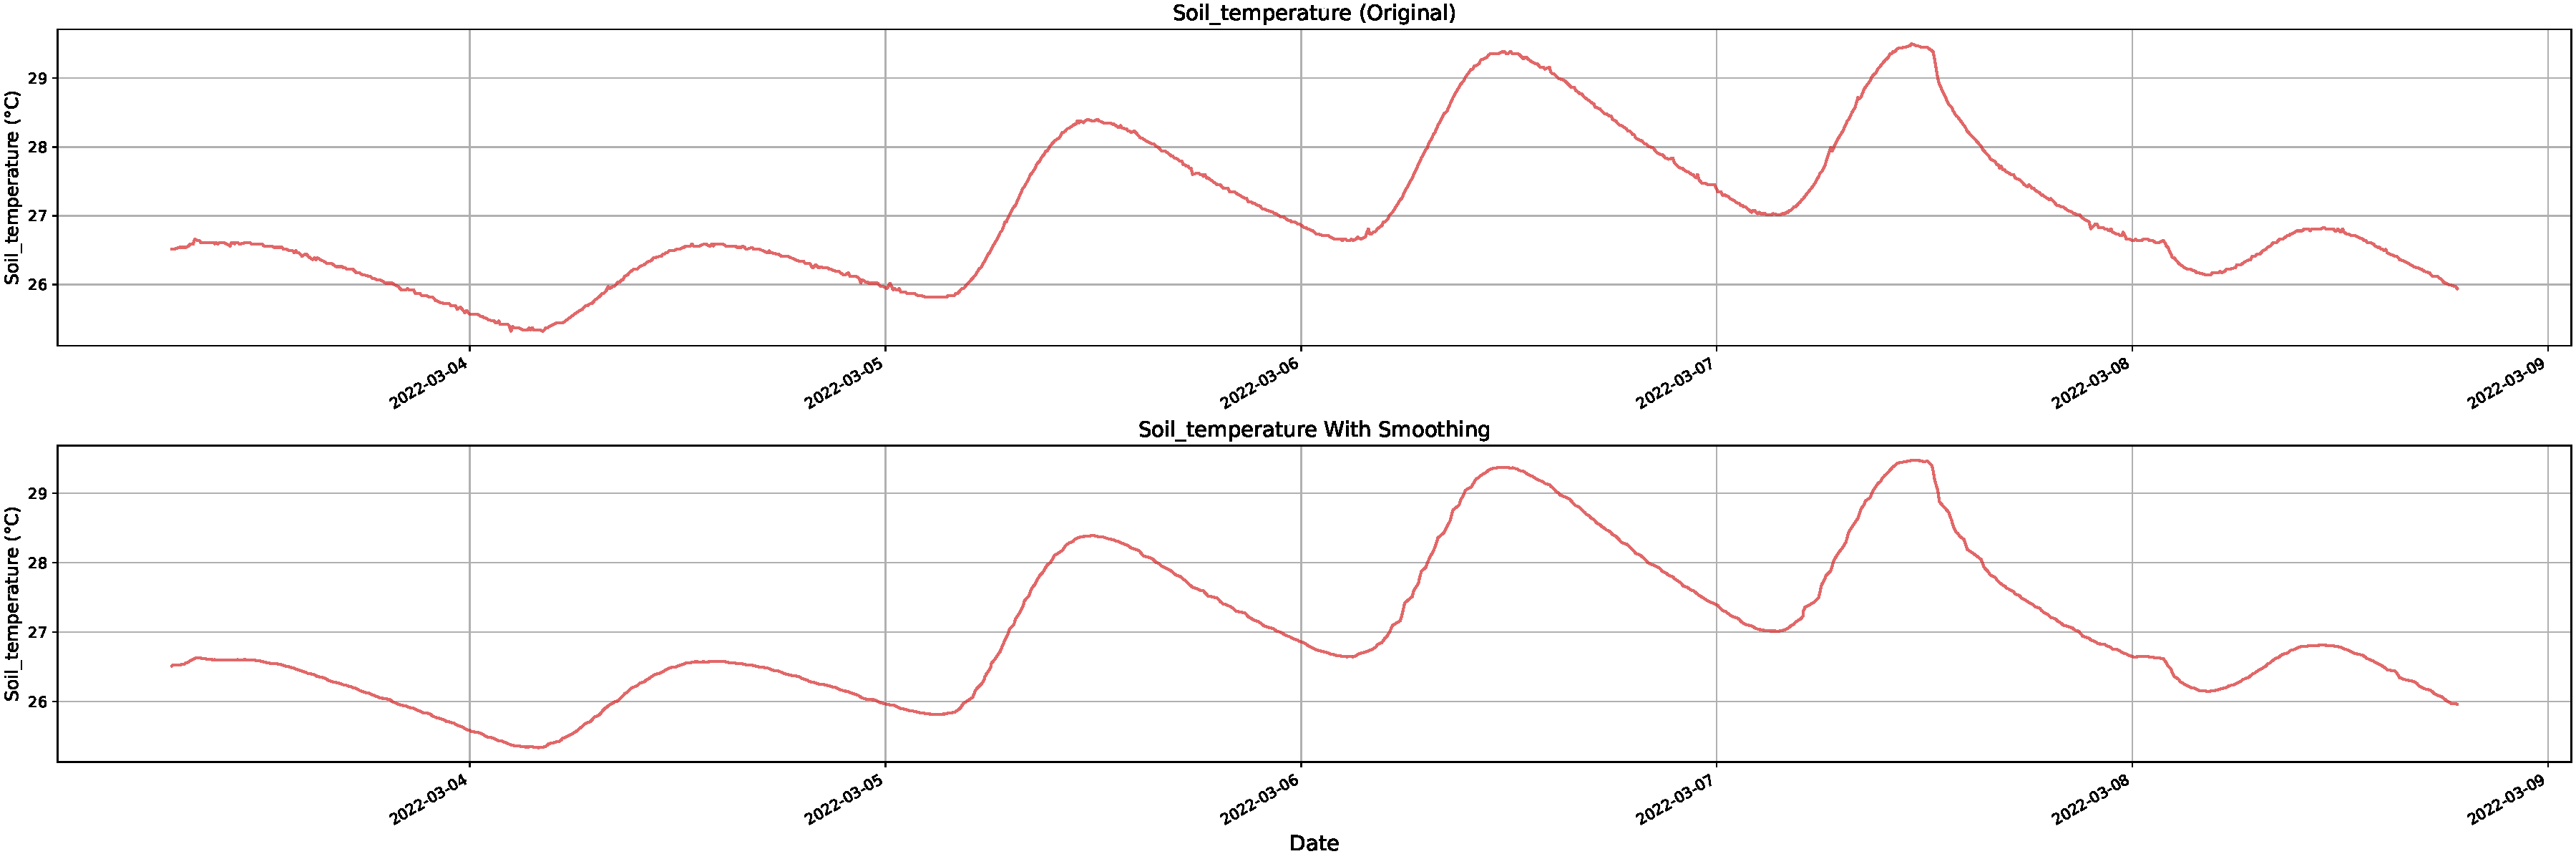
\includegraphics[width=15 cm]{5_ChapterDesign/figuras/2_Smoothing/Smoothing_Soil_temperature}
    \caption{Original Soil temperature data (top) versus the Soil temperature smoothed data (bottom) after applying a Savitzky-Golay filter}
    \LABFIG{FIG}
\end{figure}

\begin{figure}[htbp]
    \centering
    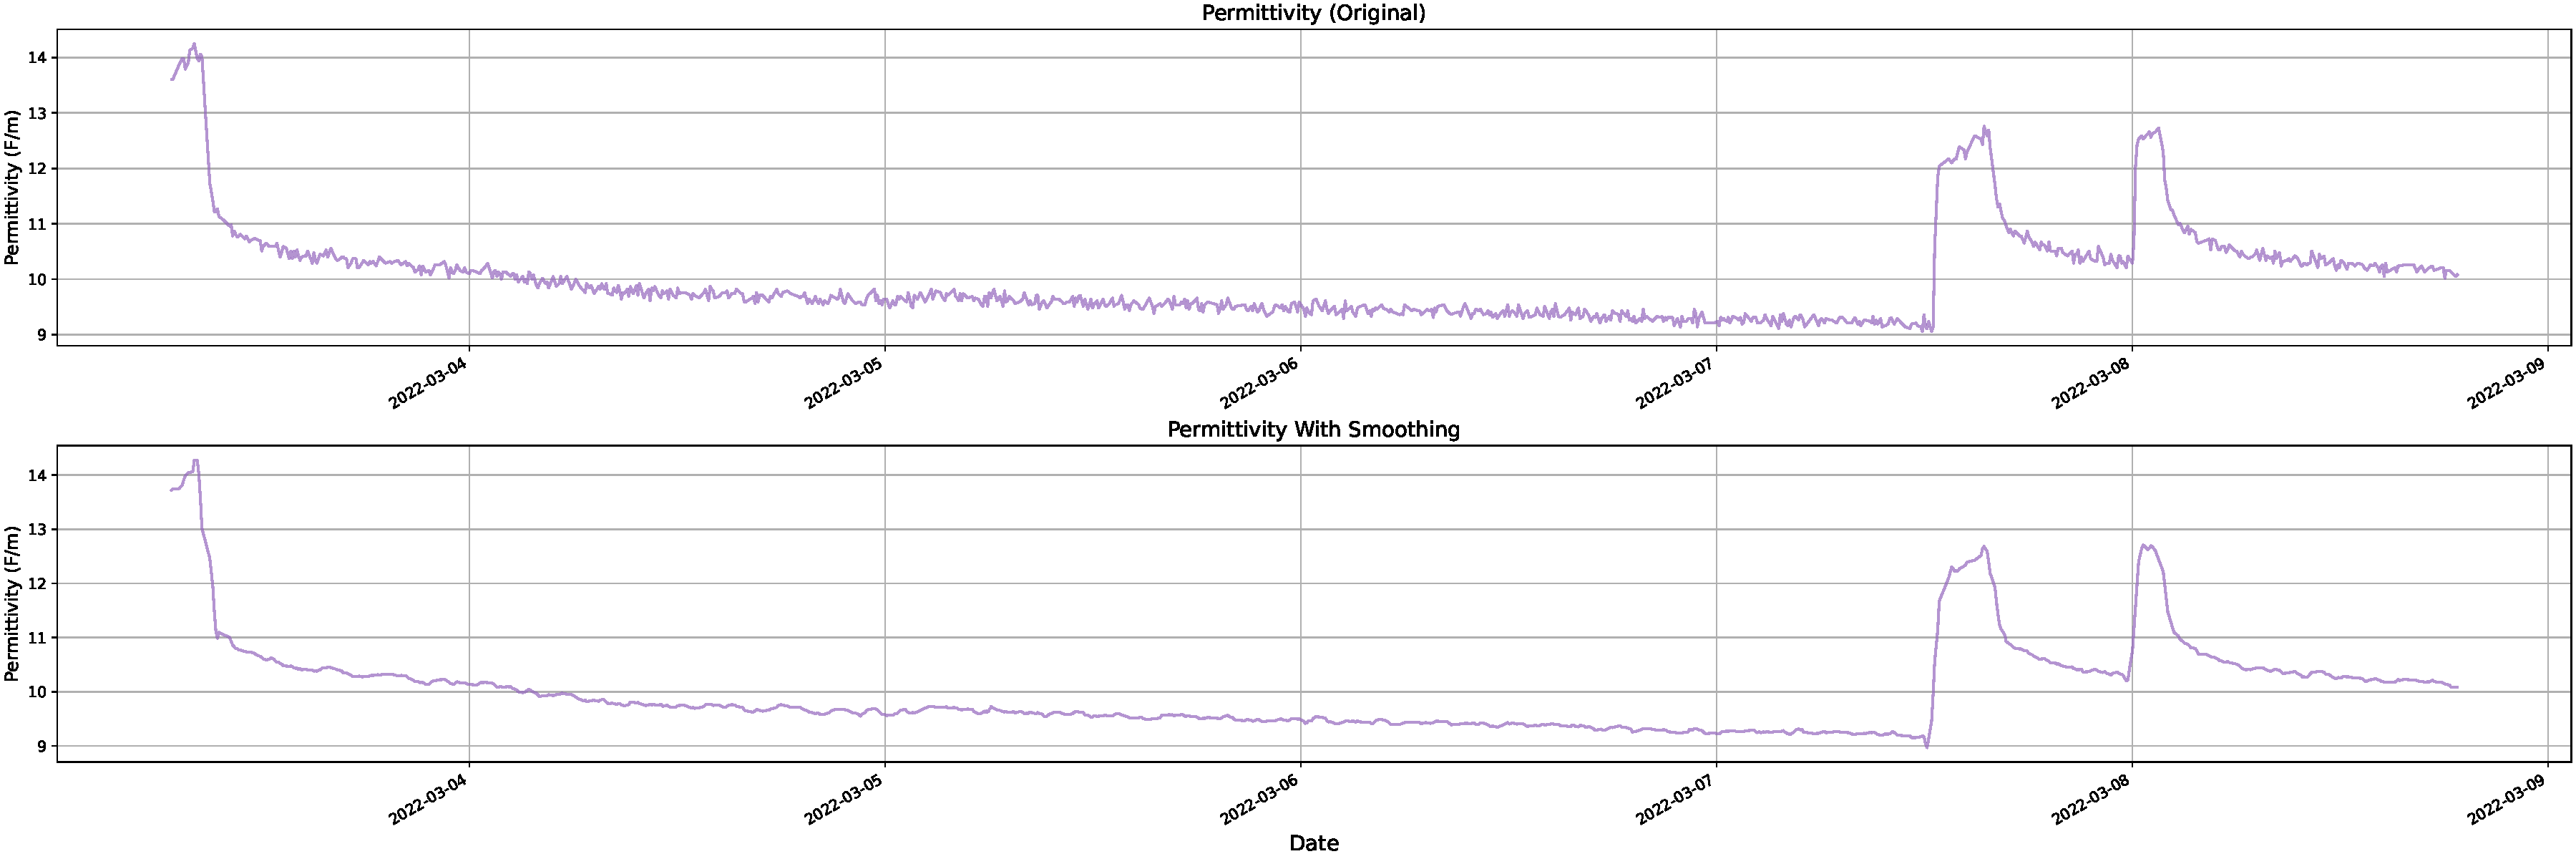
\includegraphics[width=15 cm]{5_ChapterDesign/figuras/2_Smoothing/Smoothing_Permittivity}
    \caption{Original Permittivity data (top) versus the Permittivity smoothed data (bottom) after applying a Savitzky-Golay filter}
    \LABFIG{FIG}
\end{figure}

\begin{figure}[htbp]
    \centering
    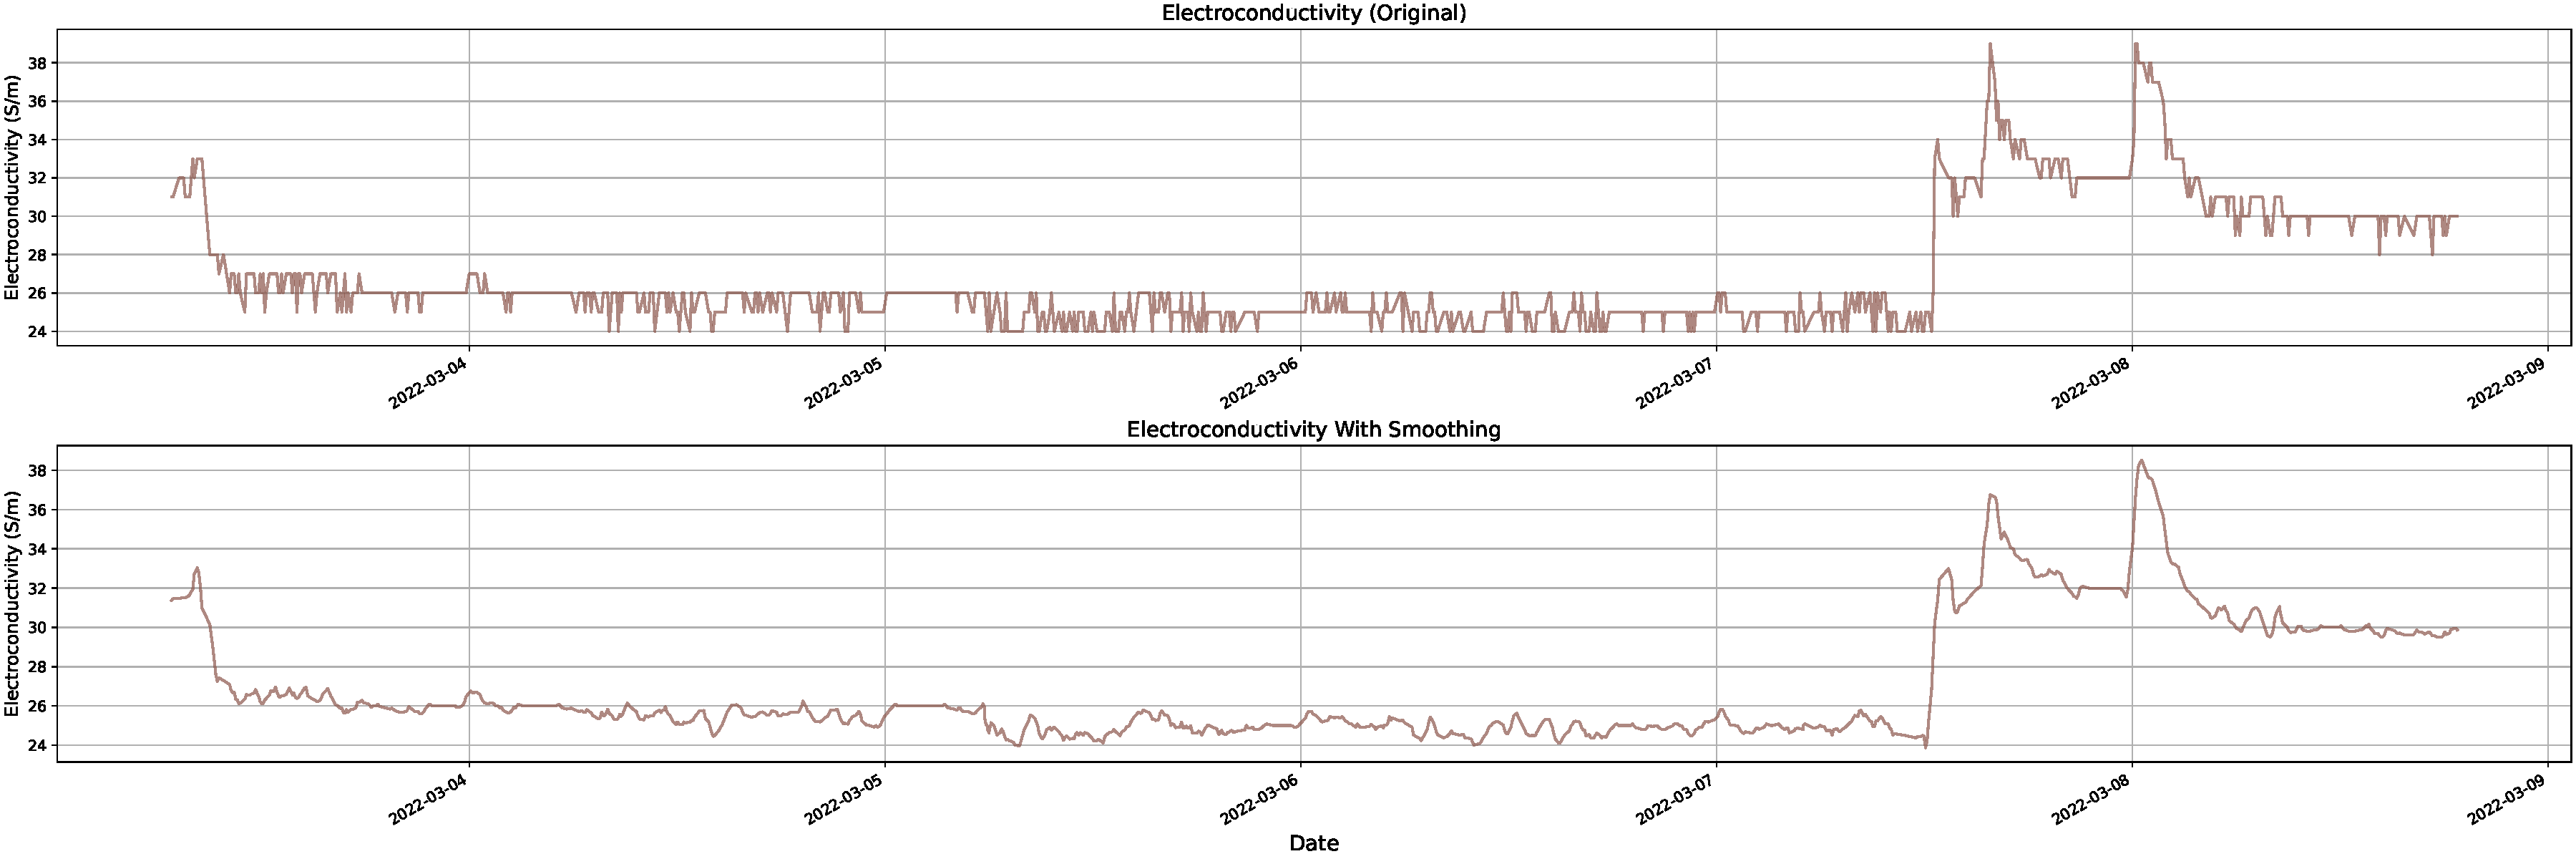
\includegraphics[width=15 cm]{5_ChapterDesign/figuras/2_Smoothing/Smoothing_Electroconductivity}
    \caption{Original Electroconductivity data (top) versus the Electroconductivity smoothed data (bottom) after applying a Savitzky-Golay filter}
    \LABFIG{FIG}
\end{figure}

\begin{figure}[htbp]
    \centering
    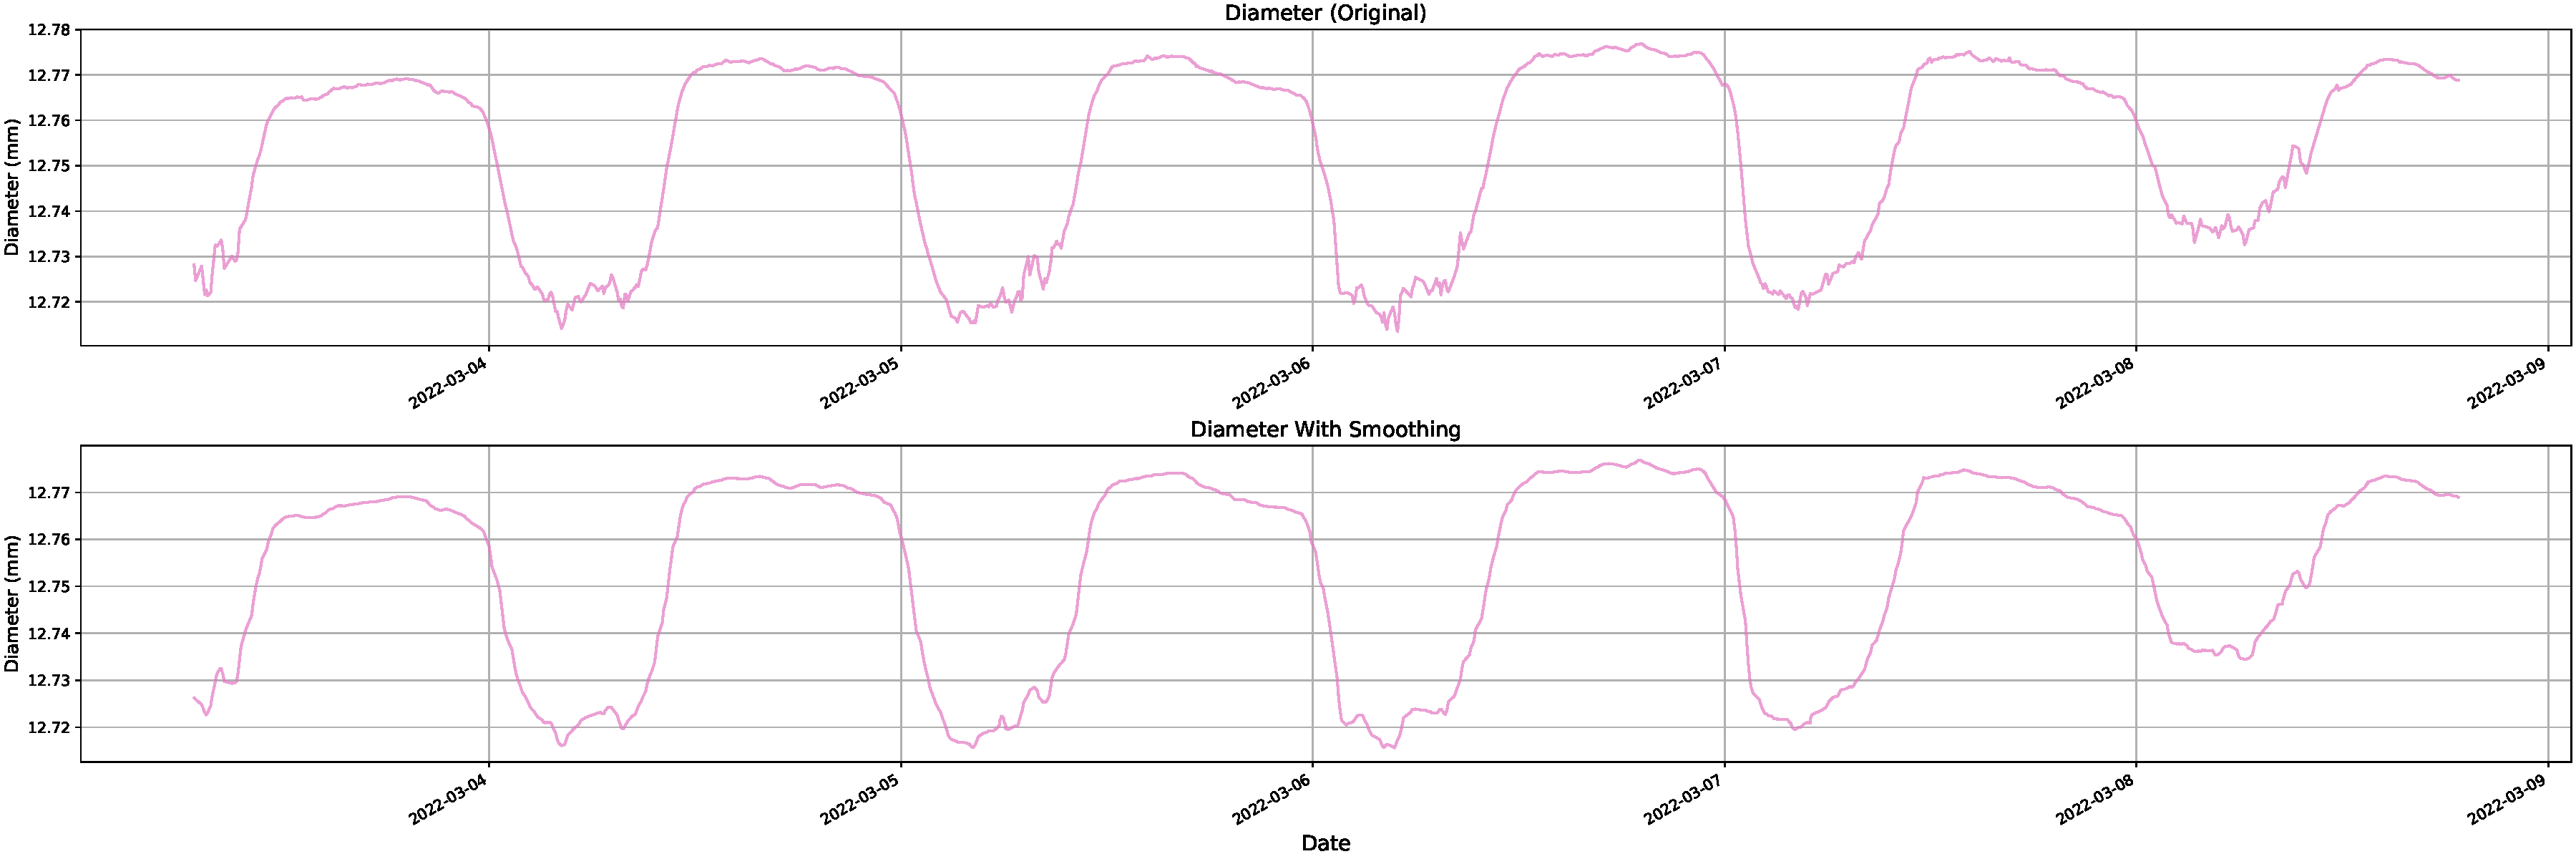
\includegraphics[width=15 cm]{5_ChapterDesign/figuras/2_Smoothing/Smoothing_Diameter}
    \caption{Original Diameter data (top) versus the Diameter smoothed data (bottom) after applying a Savitzky-Golay filter}
    \LABFIG{FIG}
\end{figure}

\begin{figure}[htbp]
    \centering
    
    % Primer par de figuras
    \begin{minipage}[b]{0.45\textwidth}
        \centering
        \begin{subfigure}{\textwidth}
            \centering
            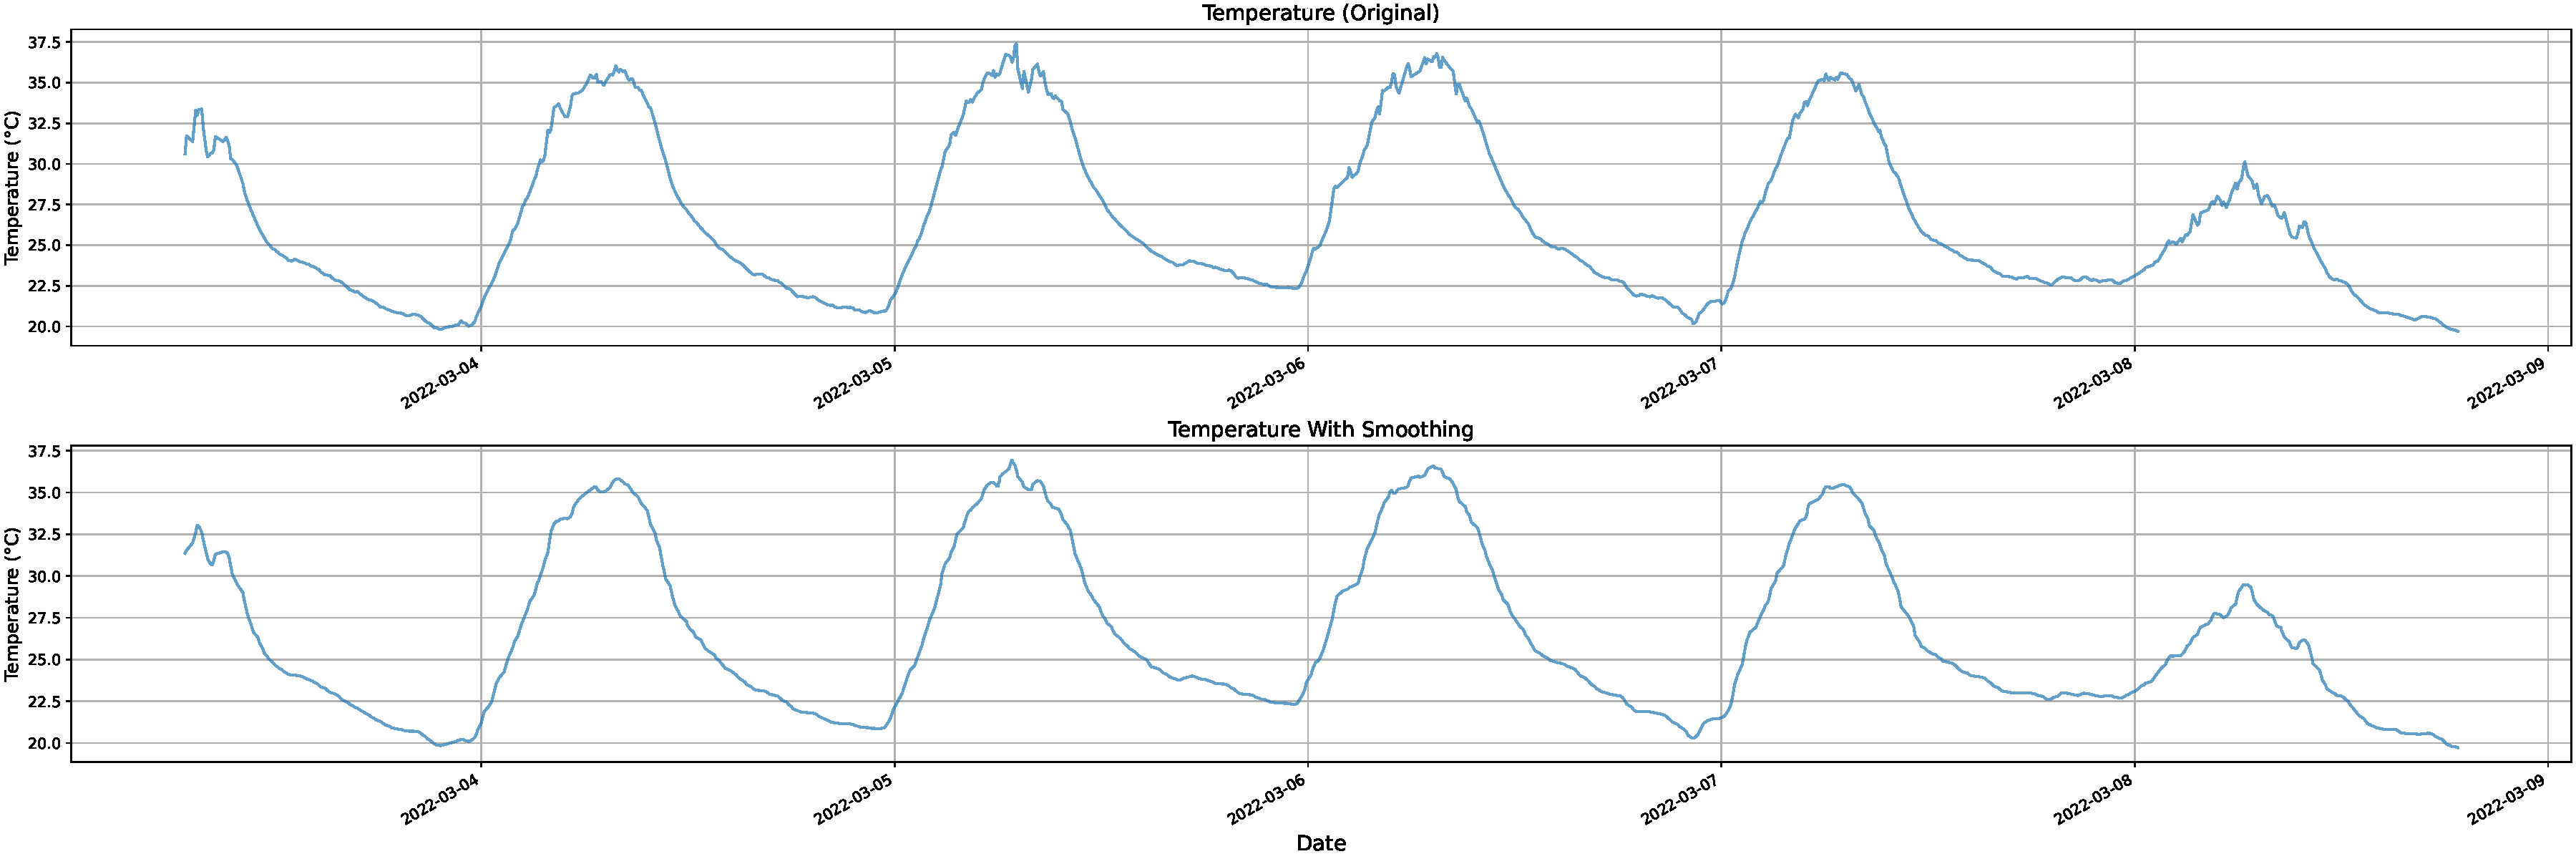
\includegraphics[width=\textwidth]{5_ChapterDesign/figuras/2_Smoothing/Smoothing_Temperature}
            \caption{Original Temperature data (top) versus the Temperature smoothed data (bottom)}
            \label{fig:temperature}
        \end{subfigure}
    \end{minipage}
    \hfill
    \begin{minipage}[b]{0.45\textwidth}
        \centering
        \begin{subfigure}{\textwidth}
            \centering
            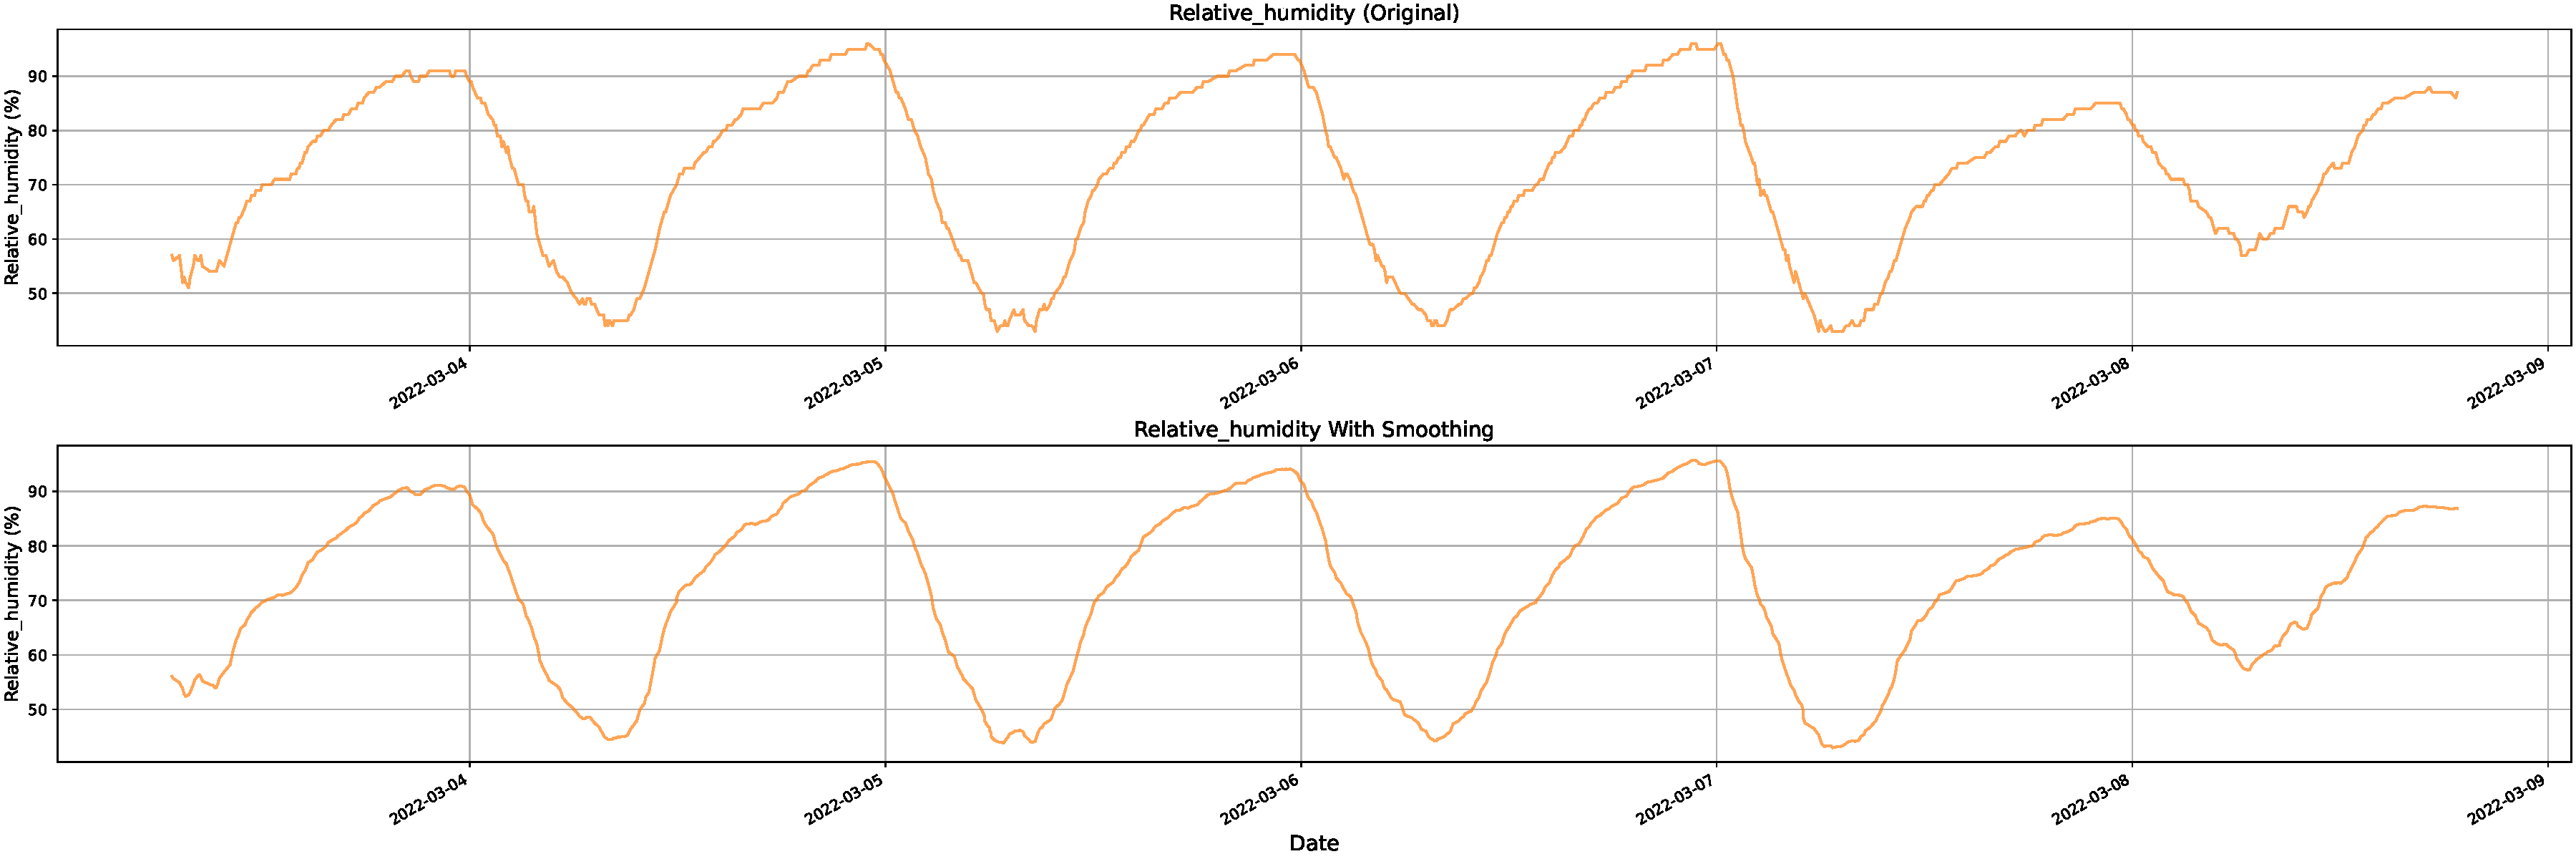
\includegraphics[width=\textwidth]{5_ChapterDesign/figuras/2_Smoothing/Smoothing_Relative_humidity}
            \caption{Original Relative humidity data (top) versus the Relative humidity smoothed data (bottom)}
            \label{fig:relative_humidity}
        \end{subfigure}
    \end{minipage}
    
    \vspace{1em}  % Espacio vertical entre las filas

    % Segundo par de figuras
    \begin{minipage}[b]{0.45\textwidth}
        \centering
        \begin{subfigure}{\textwidth}
            \centering
            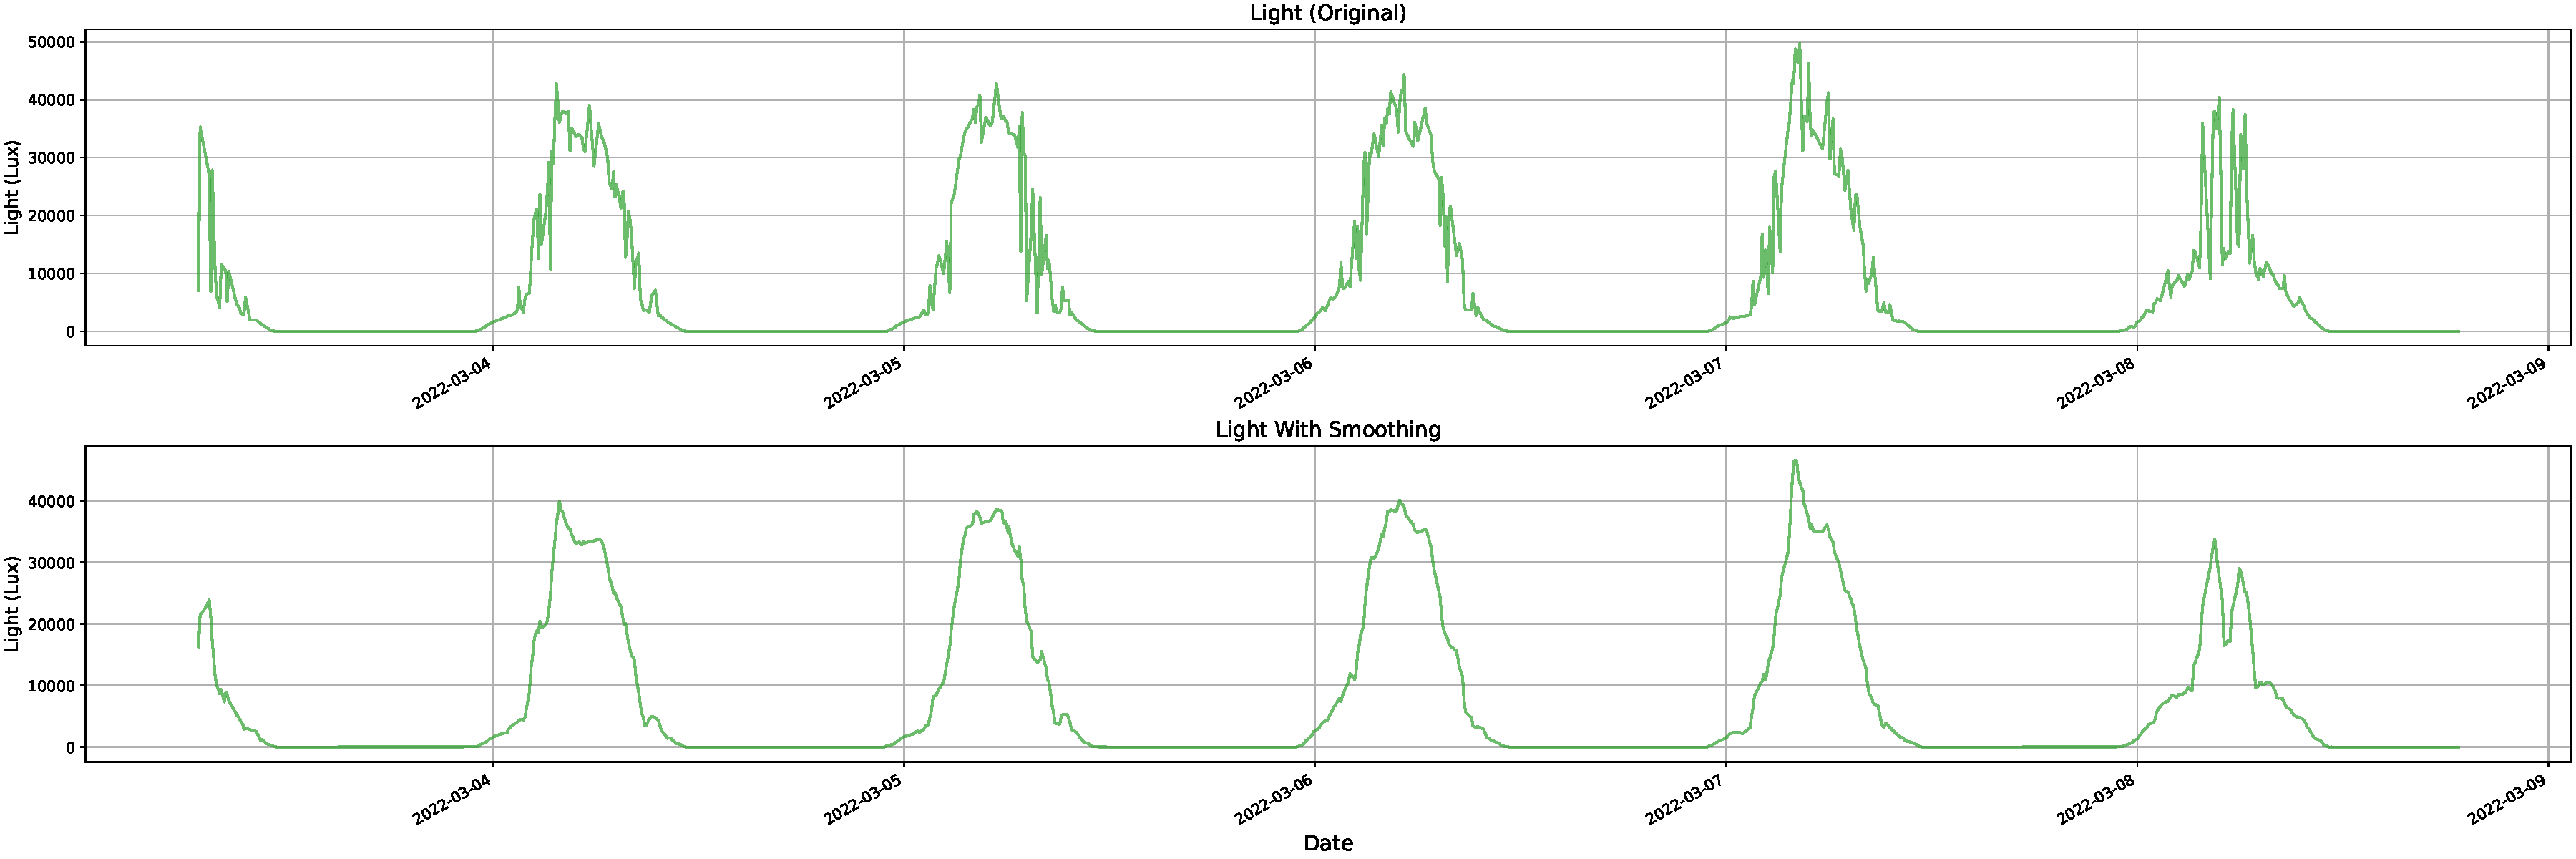
\includegraphics[width=\textwidth]{5_ChapterDesign/figuras/2_Smoothing/Smoothing_Light}
            \caption{Original Light data (top) versus the Light smoothed data (bottom)}
            \label{fig:light}
        \end{subfigure}
    \end{minipage}
    \hfill
    \begin{minipage}[b]{0.45\textwidth}
        \centering
        \begin{subfigure}{\textwidth}
            \centering
            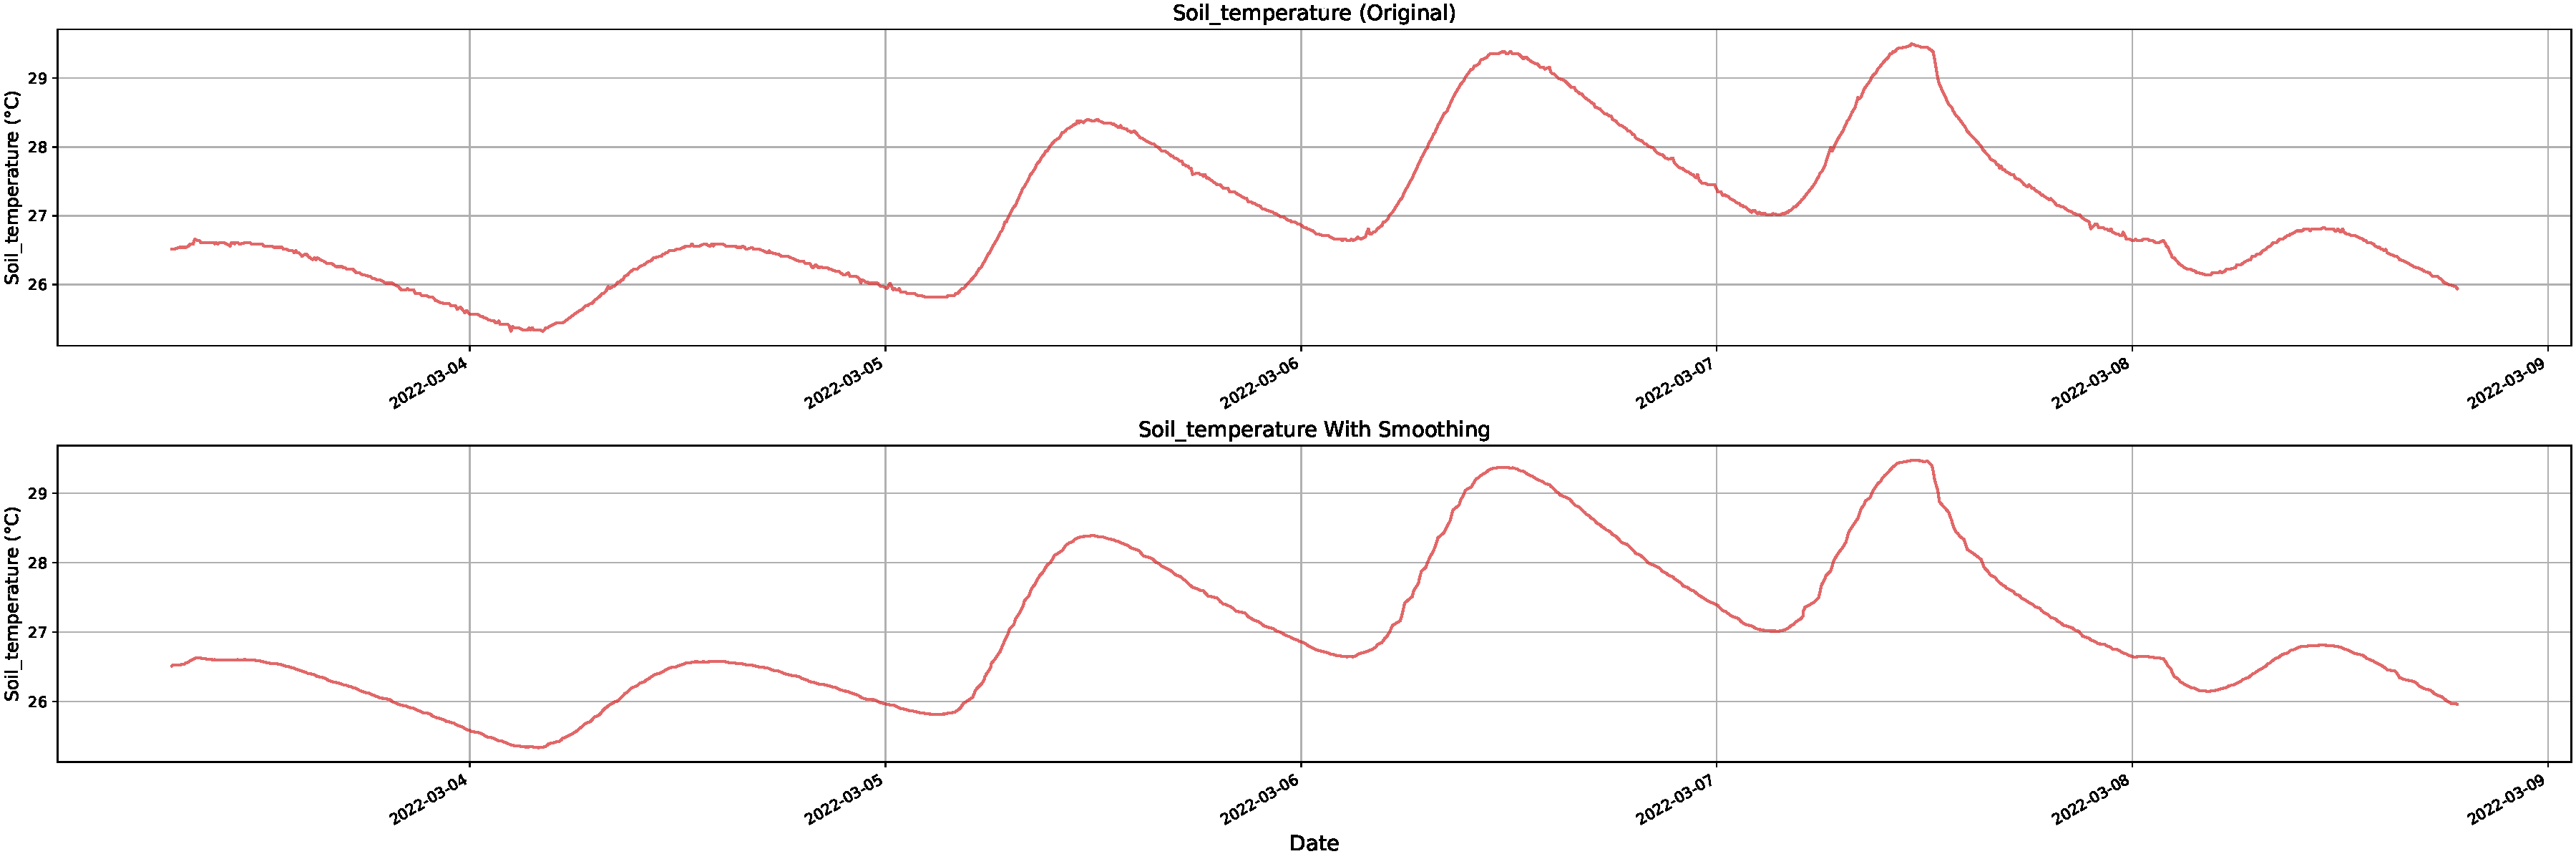
\includegraphics[width=\textwidth]{5_ChapterDesign/figuras/2_Smoothing/Smoothing_Soil_temperature}
            \caption{Original Soil temperature data (top) versus the Soil temperature smoothed data (bottom)}
            \label{fig:soil_temperature}
        \end{subfigure}
    \end{minipage}
    
    \vspace{1em}  % Espacio vertical entre las filas

    % Tercer par de figuras
    \begin{minipage}[b]{0.45\textwidth}
        \centering
        \begin{subfigure}{\textwidth}
            \centering
            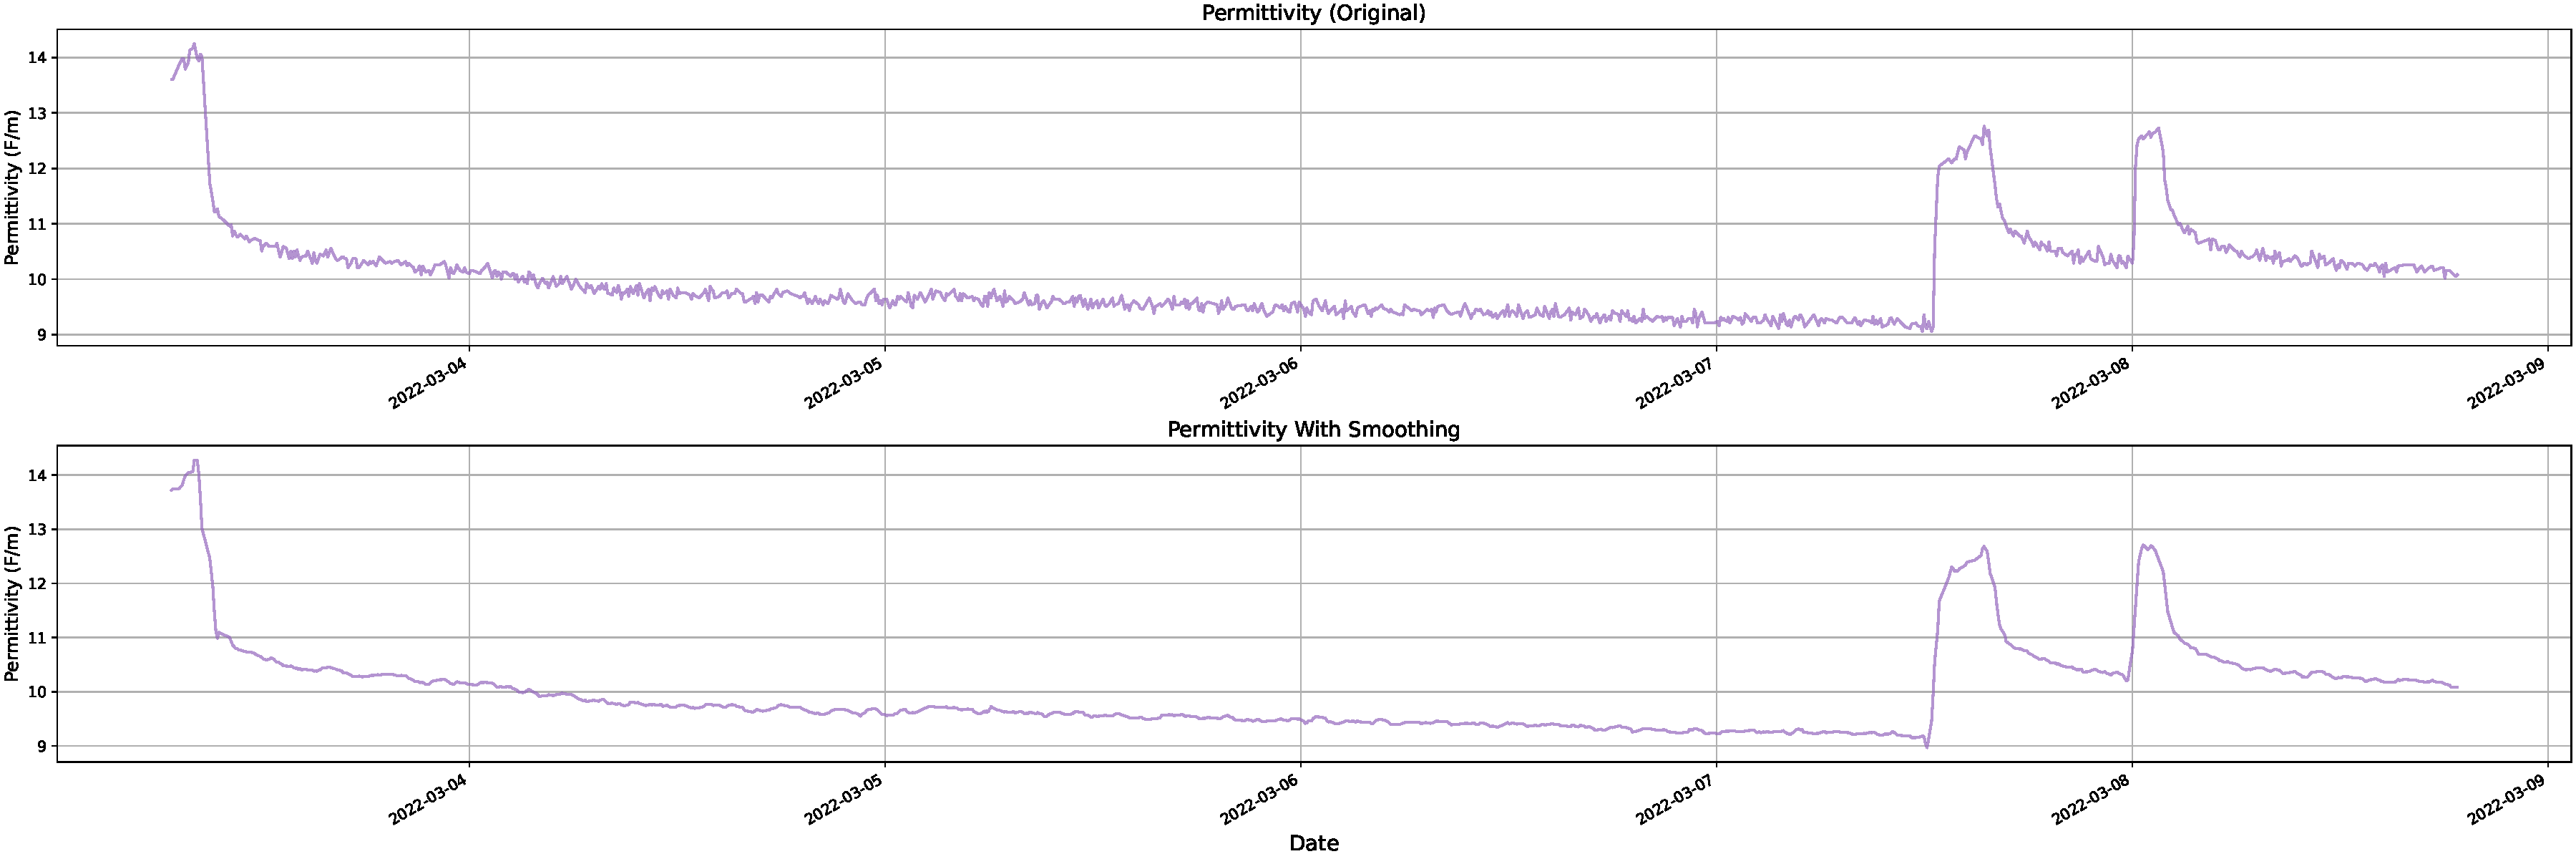
\includegraphics[width=\textwidth]{5_ChapterDesign/figuras/2_Smoothing/Smoothing_Permittivity}
            \caption{Original Permittivity data (top) versus the Permittivity smoothed data (bottom)}
            \label{fig:permittivity}
        \end{subfigure}
    \end{minipage}
    \hfill
    \begin{minipage}[b]{0.45\textwidth}
        \centering
        \begin{subfigure}{\textwidth}
            \centering
            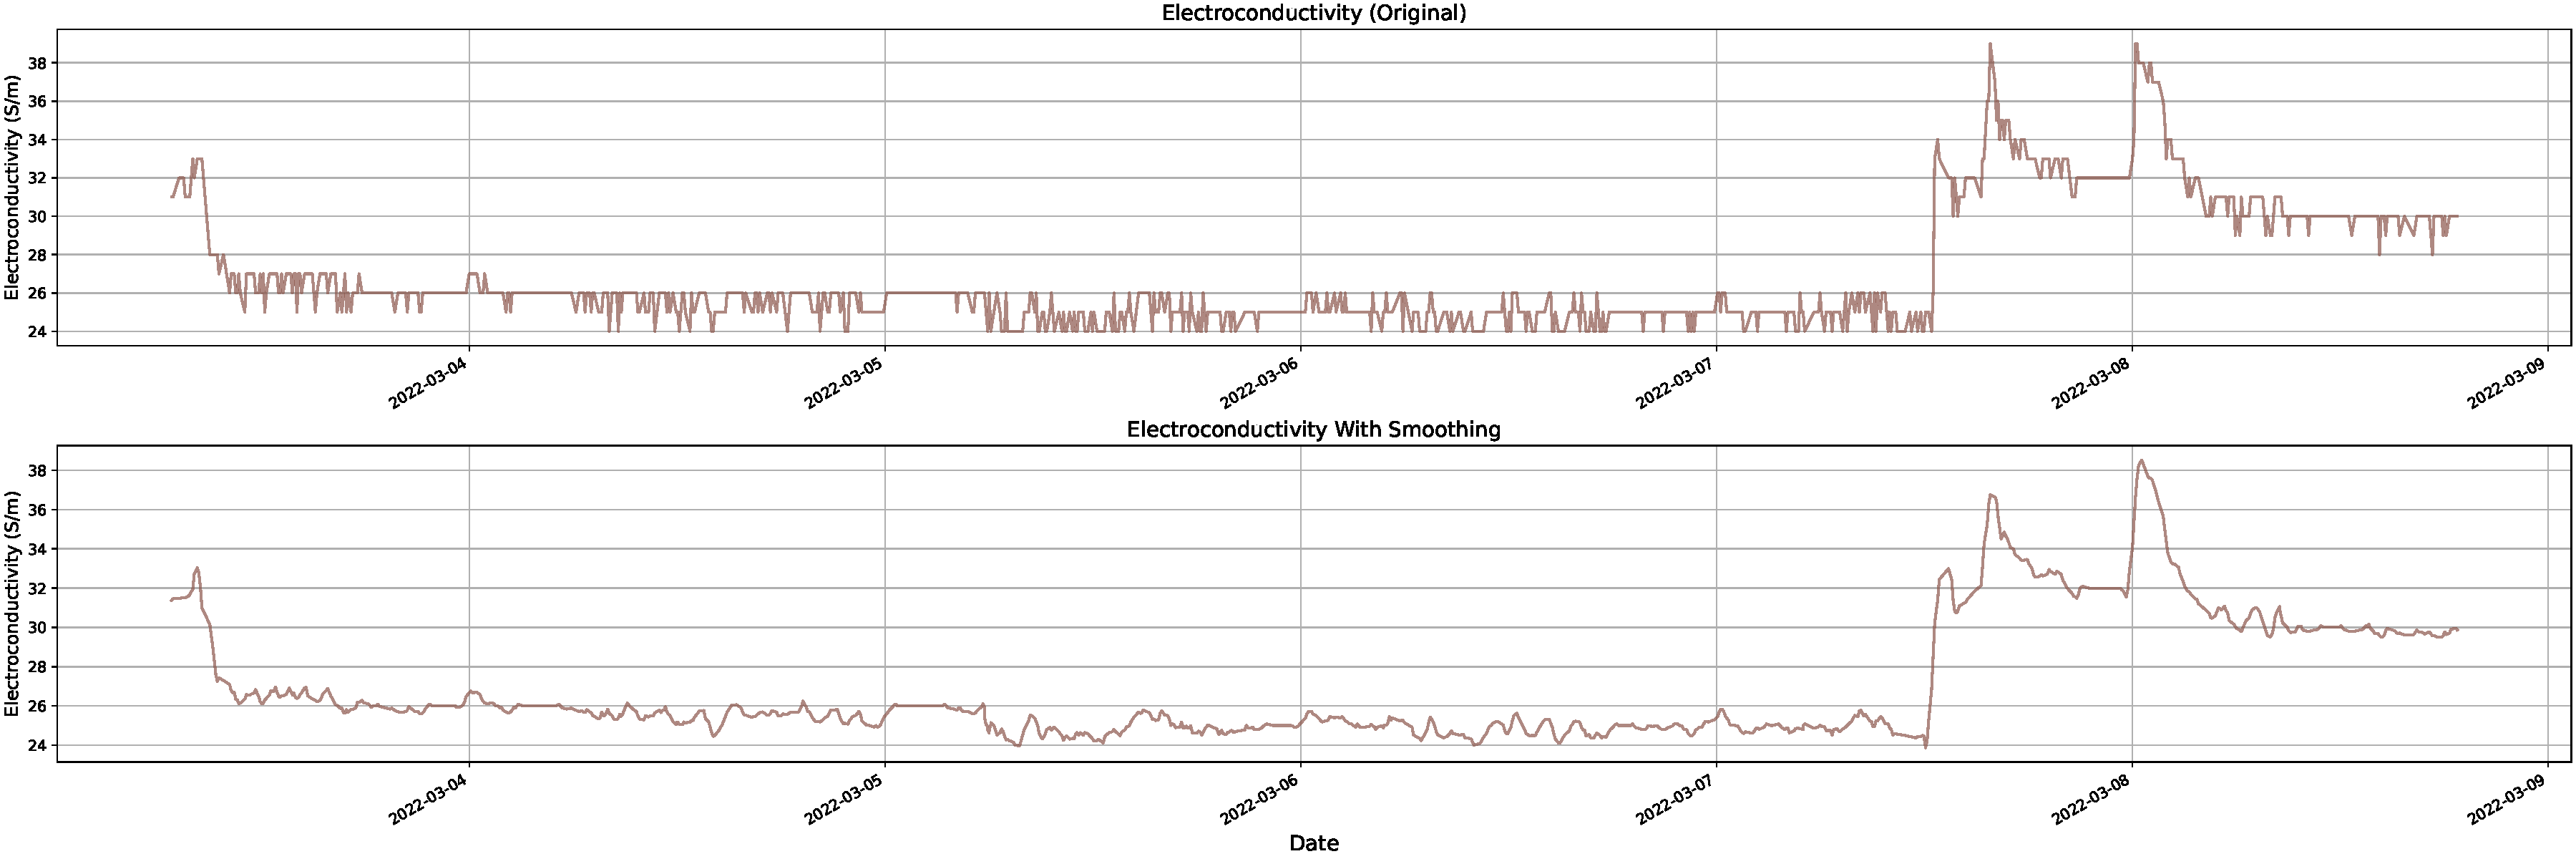
\includegraphics[width=\textwidth]{5_ChapterDesign/figuras/2_Smoothing/Smoothing_Electroconductivity}
            \caption{Original Electroconductivity data (top) versus the Electroconductivity smoothed data (bottom)}
            \label{fig:electroconductivity}
        \end{subfigure}
    \end{minipage}
\end{figure}

This type of smoothing is commonly used in signal processing to reduce noise in datasets and facilitate the identification of patterns and trends. By decreasing background noise, trends emerge more clearly, which is crucial for accurate analysis.

